\documentclass{article}%
\usepackage[T1]{fontenc}%
\usepackage[utf8]{inputenc}%
\usepackage{lmodern}%
\usepackage{textcomp}%
\usepackage{lastpage}%
\usepackage{authblk}%
\usepackage{graphicx}%
%
\title{Edwardsiella tarda Eta1, an In Vivo{-}Induced Antigen That Is Involved in Host Infection}%
\author{Michael Tate}%
\affil{Department of Pharmacology, National Medicines Institute, Warsaw, Poland}%
\date{01{-}01{-}2014}%
%
\begin{document}%
\normalsize%
\maketitle%
\section{Abstract}%
\label{sec:Abstract}%
One of the most interesting research studies in the world is performed every day on our friends in Mexico. While many others focus on researching medicinal cannabis and the marijuana{-}based virus known as Fonacase, this study suggests that the bacterium Ophiocordyceps Vella may be used as a weapon against influenza virus, as previously being seen in affected individuals. Only they can learn more from this report by looking at the importance of the bacterium called Ophiocordyceps in this particular strain of flu that is caused by H1N1.\newline%
This special report explains how data obtained by the researchers explains why and where to look to understand and correct the contributing factor in Influenza infections in U.S. Healthcare. The bacterium Ophiocordyceps Vella has shown increasing interference with normal immunocompromised population by the two influenza viruses that are affecting the population and how a viral Fonsenhimer, sometimes called M, can be consistently made in a laboratory process. However, the researchers have failed to observe any measurable increase in activity of normal H1N1 viruses.\newline%
The New York Times has commented that the paper about flu virus that is resistant to Ophiocordyceps has been published by scientists through funding from the National Institutes of Health and was as follows.\newline%
The mutation pathologist, from the Immun Immunology Center at the University of California, Los Angeles, who first identified it, Dr. Abdulkader, a member of the editorial staff of the New York Times and chief of the department of Immunobiology and Infection, said: "This paper specifically showed how there is a high interference rate that can cause the vaccine to be ineffective, it appears to have a very intense rapid antiviral effect that could affect even the most sensitive vaccine." The scientists refer to people who get a flu strain that is resistant to Ophiocordyceps Vella as "shady," referring to a trend that has been observed in the influenza subpopulations of some of the most virulent strains of the virus. Dr. Abdulkader said, "These people are obviously ill. The people are being warded away." "They are taking up to two or three times the chance of being vaccinated because of these rare resistance."\newline%
One important example of the bacterium being completely ignored during the flu outbreak period is the fact that transmission of the germs during the height of the outbreak occurred during Christmas holidays.\newline%
Only the watertight strength of a vaccine can protect against the beneficial influenza virus that causes H1N1, but a flu strain that produces a mutation that blocks normal immune response, one that requires the use of an antiviral vaccine to better protect the vaccinated population against infection, appears to be absolutely detrimental to the vaccine's effectiveness. Dr. Abdulkader has also shown that Ophiocordyceps Vella was later found to be the primary culprit in the infecting of sheep by the strains of influenza that turned up outside the Vaccine Insect Biology Laboratory of the Bassett Center for Sars Research at the University of Adelaide. The study reveals that Ophiocordyceps Vella, caused by the mutation has significantly more of a signature in the animals in question than a normal influenza virus. This creates a little traffic jam and delays antiviral transmission and difficulty in disinfecting veterinary practice. It is also noted that there are some laboratory experiments that have shown that animals left with the mutation don't pay as much attention to water as animals that don't have it.\newline%
Source:\newline%
El Sol de Mexico, The New York

%
\subsection{Image Analysis}%
\label{subsec:ImageAnalysis}%


\begin{figure}[h!]%
\centering%
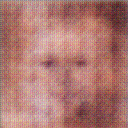
\includegraphics[width=150px]{500_fake_images/samples_5_71.png}%
\caption{A Close Up Of A Person Wearing A Tie}%
\end{figure}

%
\end{document}